\section{Introduction}
% hier das generelle minimization Beispiel rein
% was war der unterschied mit den beiden unterschiedlichen J's, wo sturmi nicht happy war?

This document was created in the context of the Computational Mathematics Seminary
at the Technical University of Vienna (SE - 3ECTS). In this introduction, the scientific relevance
of the work is highlighted and a brief overview of the topics covered is given. This overview
also follows the workflow for a generic shape optimization problem.\\

PDE Constrained Shape Optimization is a topic of interest in almost all engineering fields
where the relevant phenomena can be described by Partial Differential Equations (PDEs) and
an optimization problem can be formulated. Here, the stationary linear stokes equations are
the PDEs and the energy dissipation over the domain is optimized. The optimization can 
be described by a minimization problem which can be solved with the gradient descent method.
Its important to note here, that the PDE constraints and optimization goals used here, 
can be exchanged with arbitrary PDE constraints and optimization goals. Some parts,
especially the proof for shape derrivative existence, can get more complex for e.g. 
Non-Linear PDEs or Transient PDEs.\\

\subsection*{Minimization Problem}
A generic PDE constrained optimization problem is of the following form:

\begin{align*}
        \min_{ \Omega \in \mathcal{A} } J( \Omega, u) \\
        : \mathrm{B}_{\Omega}(u) = 0
\end{align*}

Where $\Omega$ is the Domain for the PDE, $\mathcal{A}$ is the set of admissible shapes
$J(\Omega, u)$ is a functional that is to be minimized and $\mathrm{B}_{\Omega}(u)$ is the PDE
constraint and its solution $u$. The Domain $\Omega$ is what is going to be 
optimized in the underlying work. \\

\subsection*{Shape Derrivative}
In order to find a numerical solution to the minimization problem with the gradient descent
method, the existence of the analytical shape derrivative needs to be shown. Here the
differentiability of $J(\Omega,u)$ at $\Omega \in \mathcal{A}$ in direction $X$ is shown. 
As Sturm et. al. \cite{nearly_conformal_paper} have shown, the functional 
$J(\Omega, u)$ can be reduced to a functional $J(\Omega)$ and the shape derrivative 
$\mathrm{d}J(\Omega)(X)$ exists. In chapter \ref*{}, the proof is recapitulated briefly.

\subsection*{Auxiliary Problem - Descent Direction}
To find the gradient descent direction, here the vectorfield $-X$, an auxiliary problem needs to be solved.
Since its solved with the Finite Element Method libary NGSolve, the PDE problem is posed in a weak sense where 
$H$ is e.g. a Sobolov space.find $X \in [H(\Omega)]^2:$ 
\begin{align*}
    \mathrm{d}J(\Omega)(X) = \mathrm{b}(X,\varphi)_H \quad \forall  \varphi \in H
\end{align*}

If the bi-linear form $\mathrm{b}(.,.)_H$ is chosen such that it is positive definite, the negative solution $X$
of the auxiliary problem points in the negative direction of the gradient.

\pagebreak

\subsection*{Optimization Steps}
The Stokes Equations on the initial domain are solved, the cost functional $J(\Omega)$



i want to cite \cite{fully_semi_paper_sturm}
and also \cite{vol_bary_constraint_paper} and also \cite{lecture_notes_sturm} and also \cite{nearly_conformal_paper}, 
A figure example and a text where I refer to figure \ref{shape_opt_plot} below! Additionally I need other citations like \cite{lecture_notes_faustmann_numPDE}
as well as \cite{lecture_notes_faustmann_AMF} and \cite{lecture_notes_melenk_numcomp}
yes yes yes or no? David Kempf
\begin{figure}[ht]
    \centering
    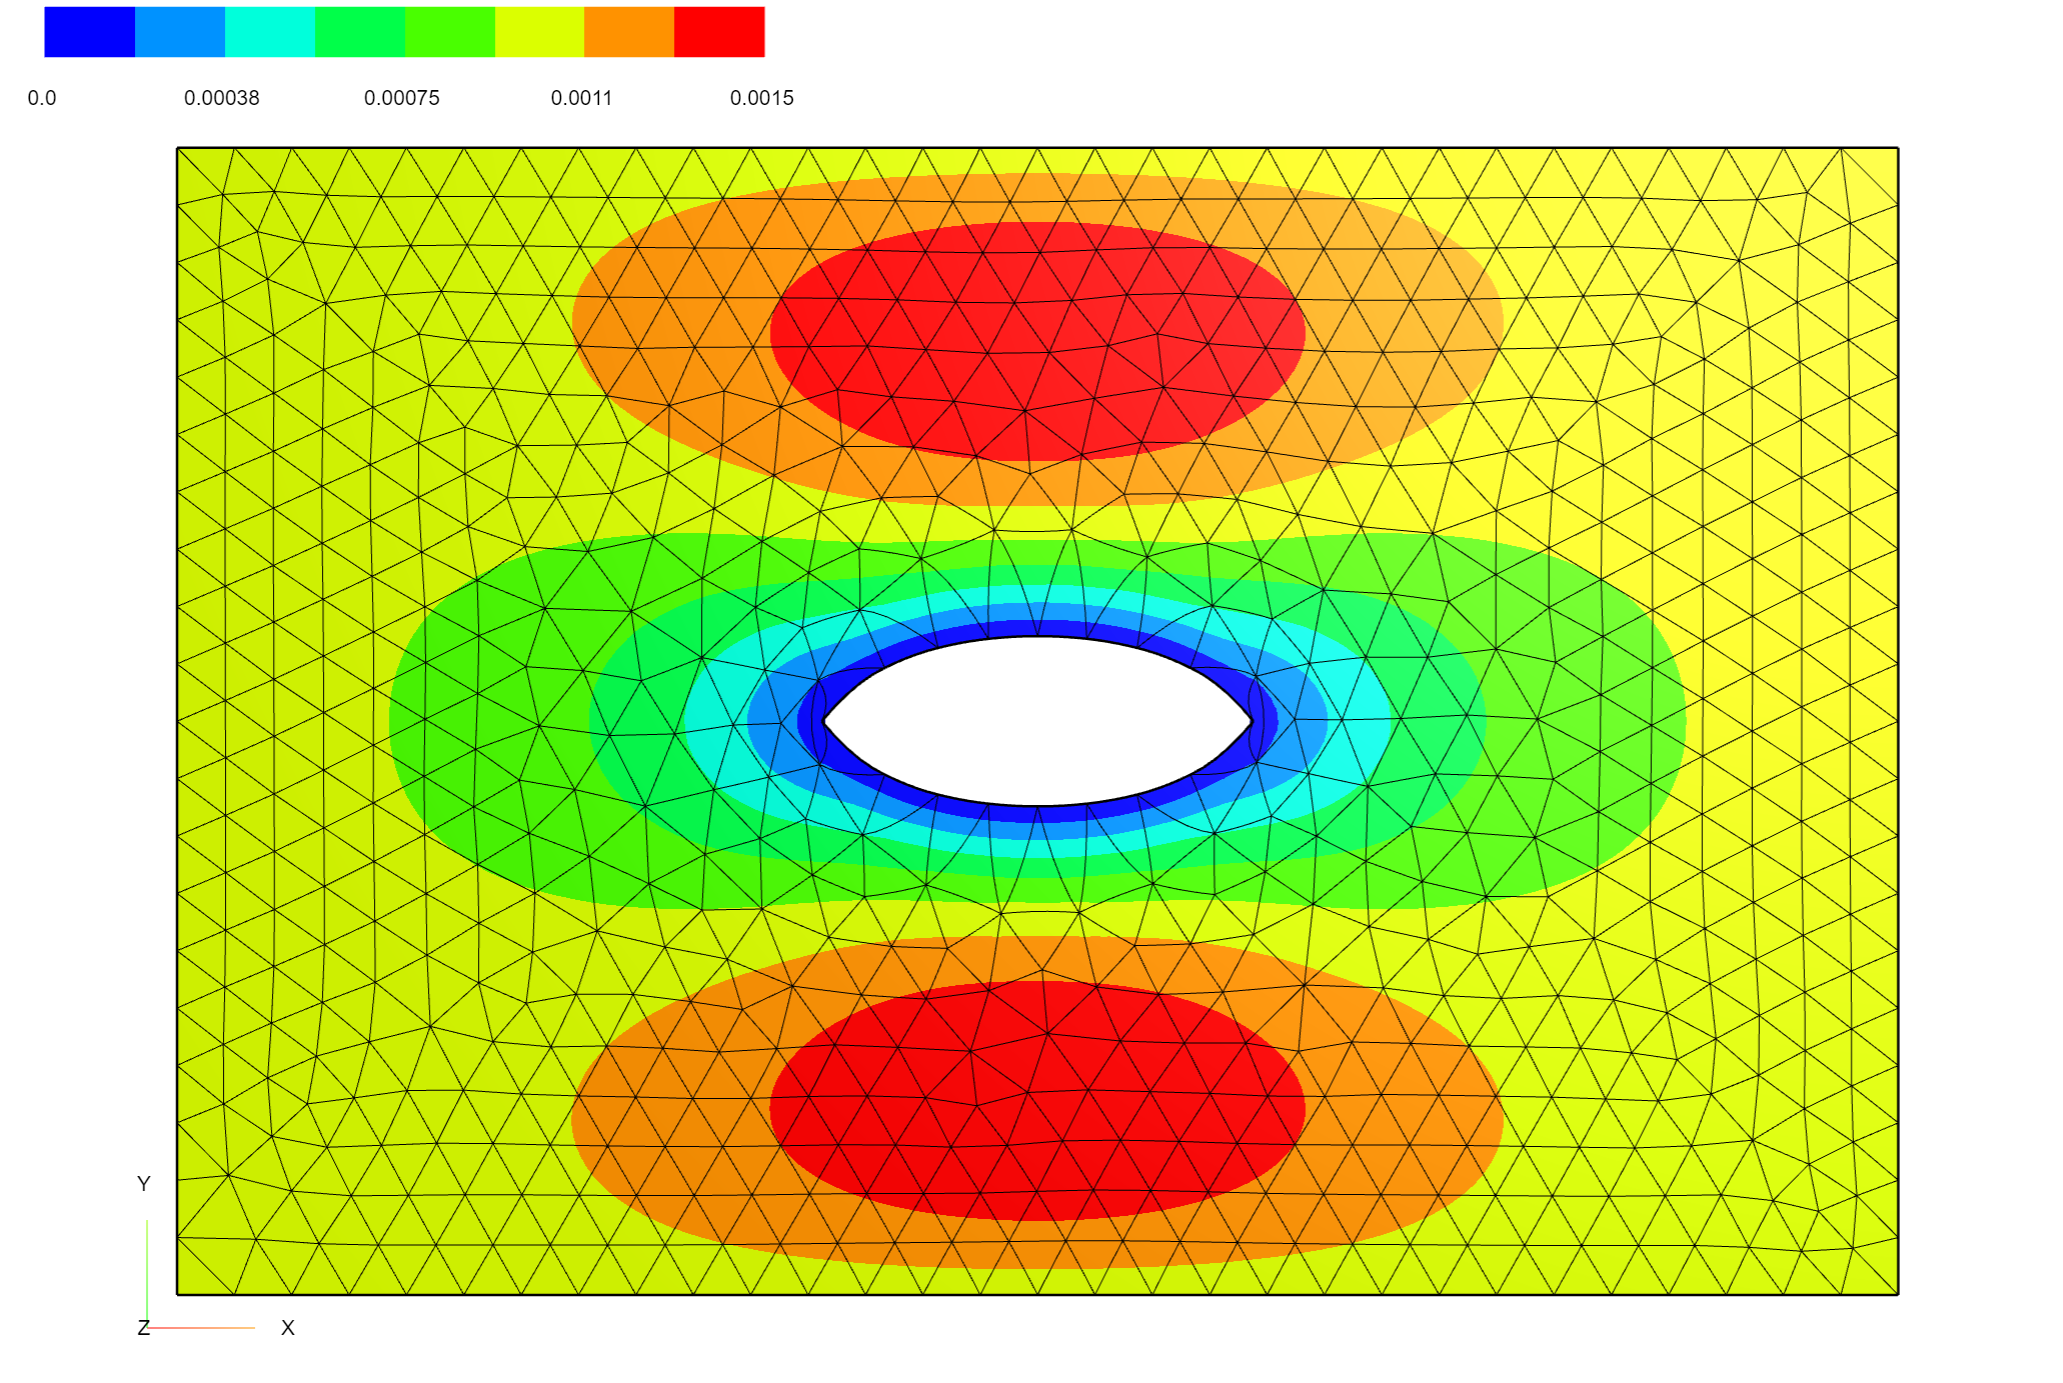
\includegraphics[width=0.8\textwidth]{figures/solution_shape_opt.PNG}
	\caption{Velocity magnitude of Stokes flow after shape optimization}
	\label{shape_opt_plot}
\end{figure}

\begin{figure}[ht]
    \centering
    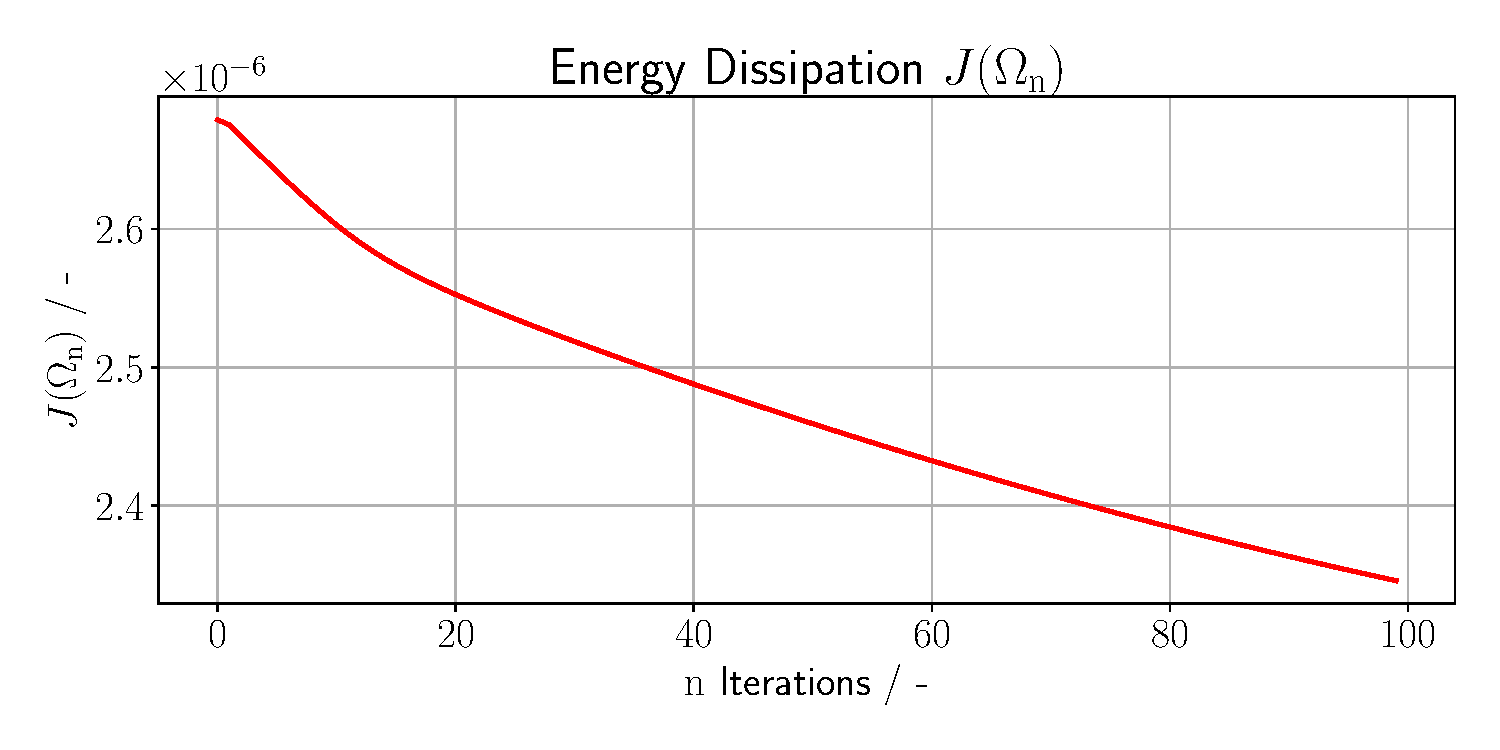
\includegraphics[width=0.8\textwidth]{figures/energy_diss_plot.pdf}
	\caption{Velocity magnitude of Stokes flow after shape optimization}
	\label{shape_opt_plot}
\end{figure}